\documentclass[DIV=calc, paper=a4, fontsize=11pt]{scrartcl}	 
\usepackage[english]{babel} 
\usepackage[svgnames]{xcolor} 
\usepackage{fix-cm}	 
\usepackage{fancyhdr} 
\pagestyle{fancy} 
\usepackage{lastpage} 
\usepackage{wrapfig}
% Header and  Title page 
\lhead{Floss Leader}
\rhead{Mater on libre software }
\cfoot{}
\rfoot{\footnotesize Page \thepage\ of \pageref{LastPage}} % "Page 1 of 2"

\renewcommand{\headrulewidth}{0.0pt}
\renewcommand{\footrulewidth}{0.4pt} 
\usepackage{titling} 
\newcommand{\HorRule}{\color{DarkGoldenrod} \rule{\linewidth}{1pt}} % 
\pretitle{\vspace{-30pt} \begin{flushleft} \HorRule \fontsize{50}{50} \usefont{OT1}{phv}{b}{n} \color{DarkRed} \selectfont} 
\title{Matthias Ettrich}
\posttitle{\par\end{flushleft}\vskip 0.5em} % Whitespace under the title
\preauthor{\begin{flushleft}\LARGE \lineskip 0.5em \usefont{OT1}{phv}{b}{sl} \color{DarkRed}} 
\author {Amal Roumi,} 
\postauthor{ \usefont{OT1}{phv}{m}{sl} \color{Black}University Ray Juan Carlos 

\par\end{flushleft}\HorRule} 

\date{}

%----------------------------------------------------------------------------------------

\usepackage{graphicx}
\usepackage{amsmath}
\begin{document}
\maketitle
\thispagestyle{fancy} % Enabling the custom headers/footers for the first page 

\begin{center}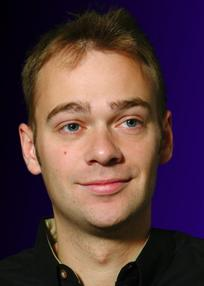
\includegraphics[scale=1.5]{index.jpeg} \end{center}

%------------------------------------------------------
\abstract
\textbf{Summary} \\
 
As a part of my assignment in subject Developers and Motivations for master in libresoft, we have studied some of the most important leaders in the world of free software.
 This report will talk  about one of these FLOSS leader ..\emph{Matthias Ettrich}
 \\

\tableofcontents
 \newpage

%------------------------------------------------------
\section{Biography \& Background}

Matthias Frank Ettrich is a computer scientist born 14 June 1972 in Bietigheim-Bissingen, southern Germany.\\

{\Large \textbf{\emph{Education}}}
He earned  Master's degree,in Computer Science graduating from Eberhard Karls University Tuebingen\footnote{http://www.uni-tuebingen.de/en/university.html}. in 1989, and his Matriculation was from  Herzog-Christoph-Gymnasium Beilstein \footnote {http://www.hcgbeilstein.de/}\\

{\Large\emph{\textbf{Career}}}\footnote{http://www.linkedin.com/pub/matthias-ettrich/28/9b0/aa8}
His early works was at 1998  as Senior Software Engineer in Trolltech, developed the first graphical installer ever for the Linux Operating System (Caldera OpenLinux Lizard).by 2000 effectively lead the team,he planned, executed and partially developed Qt Designer, Trolltech's first visual GUI design tool .after two years he became Director of Software Development ,then as VP Engineering.
after Trolltech were acquired by Nokia and opened a German R\&D office for Trolltech he was the Managing Director while he still functioning as VP of Engineering for the global operations.later he was Head of R\&D Germany Nokia then Head of Development.

Now he currently  works for Nokia as Head of Architecture in Berlin, Germany on the Qt graphical widget toolkit and the Qt Creator IDE. 

%-------------------------------------------------------------

\section{ Contributions and Achievements}

Matthias Ettrich is creator of Lyx Text Processor , Founder of the KDE desktop environment .
 
 In 2009, Ettrich was  recieved German’s highest civil general decoration — the German Federal Cross of Merit \footnote {http://matija.suklje.name/matthias-ettrich-awarded-the-german-federal-cross-of-merit} for his contributions to FOSS \\
 Acorrding to Ohloh Ettrich contribute in KDE project around 23.5\% of the comment , 84,567 line changed from 1997 to 2009 .
 %---------------------------------------------------------------------------
\subsection{LyX}

Ettrich started developing a shareware graphical  front-end  program to LaTeX called Lyrix in 1995.before renamed to  \emph{  \textbf{LyX}  document processor that encourages an approach to writing based on the structure of the documents (WYSIWYM) and not simply their appearance (WYSIWYG)}.\\
 It was then announced on USENET \footnote {an early non-centralized computer network for the discussion of particular topics and the sharing of files via newsgroups.}, where it received a great deal of attention in the following years.

Matthias Ettrich comments in interview .
\begin{quote}
\emph{"Although the project really didn't stop the success of Word, it turned into a successful free software project with an active development community, and it taught me how free software projects work internally"}\footnote {http://www.linuxjournal.com/article/6834}
\end{quote}

LyX's main target platform was Linux, so he started to explore different ways to improve the graphical user interface, which ultimately led him to the KDE project. and because he found good programming team for LyX development he  focused on KDE and leave the Lyx
\begin{quote}
\emph{"I was still envolved a lot in the LyX development at this time. But since LyX found an excellent programming team I could easily do something else without any fear that the LyX development might slow down"}\footnote {http://www.linux-center.org/articles/9809/interview.html}
\end{quote}
%---------------------------------------------------------
\subsection{KDA}
The KDE project started on October 14th 1996.
KDE stands for Kool Desktop Environment.
 powerful graphical desktop environment for Unix workstations. You can think KDE as a GUI for Linux OS. KDE provides Linux users a graphical interface to choose their own customized desktop environment.
 from the KDE Project Announced 
\begin{quote} "One of the major goals is to provide a modern and common look\&feel for all the applications. And this is exactly the reason, why this project is different from elder attempts." \footnote {From the KDE Project Announced {http://www.kde.org/announcements/announcement.php}}
\end {quote}
KDE has lots of application and tools, in order to provide users all the tools they need.
for office,internet multimedia, games, educational, system, utilities, graphics, development.\\
The KDE project serves as an umbrella project for many standalone applications and smaller projects that are based on KDE technology.
\subsubsection {KDE Community}
The main features of KDE Community are:\\
KDE does not have a single 'benevolent dictator' who can veto important decisions. Instead, at KDE  team consisting of several  contributors takes decisions on the basis of merit and consensus building in Lots of small sub-communities (kdegames, kdeedu, amarok, etc.).
The  KDE community has many countries, KDE has local branches. These are either informal organizations like (KDE India) or given a legal like  (KDE France). The local organizations host and maintain regional websites, and organise local events  contributor meetings and social community meetings.
This team communicates using the  mailing list, and IRC for which is publicly archived and readable  and  the forums for users .In multiple areas: translators, artists, usability people, testers, documentation writers, promoters, packagers, developers.it is friendly to new people.
The KDE community is the second largest Free Software community behind the Linux kernel community .
%--------------------------------------------
\subsubsection {Matthias role within KDE}
After he founded the project, he was busy with  the terminal emulation, the window manager, the desktop panel, session management ,working on the libraries (DCOP) managed to turn GNU/Linux into a serious contender on the desktop ,managed to maintain a strong and growing developer and user community.
but later Matthias did not do  KDE coding work .Everything he has been doing goes into Qt. But since Qt is a part of KDE, or KDE a superset of Qt,he still consider as a KDE programmer.
.\footnote {From interview by  Swapnil Bhartiya - Feb 18, 2012}
%---------------------------------------
\subsubsection{KDE Worlds events}

Teams of development in KDE work mostly independent and do not all follow a common release schedule, there are many people working with and in several teams.  all share a common purpose and a common passion,  and they meet  together at least once a year at \textbf{Akademy}  which takes place in or close to Europe while \textbf{Camp KDE} is a north-American event,and more of events around the world.
\textbf{Developer Sprints} which focused gatherings of developers to work on a specific part of KDE\\
The success of the project for sure is result of collaboration between the community and their leaders like Matthias.

%----------------------------------------
\subsection{ QtMozilla}
The Mozilla toolkit has a backend that uses the Qt application and UI framework from Nokia
Ettrich participated to QtMozilla, helped by writing code and documentation, and by testing.
\begin {quote}
" We have been able to replace around 500 thousand lines of code with about 25 thousand lines of Qt based code - in just one week" \footnote{http://www.linux-center.org/articles/9809/interview.html}
\end {quote}

He contributed too with the KOffice development, that plays an important role in actually making Open Document a real standard.

%---------------------------------------

\section{Contact Informations }
\begin {itemize}
\item \textbf{LinkedIn}: http://www.linkedin.com/pub/matthias-ettrich/28/9b0/aa8 
\item \textbf{Qt Blog} http://blog.qt.digia.com/blog/author/ettrich/
\item  \textbf{Google+\ } https://plus.google.com/101672028461854882770/posts
\item \textbf{Facebook} https://www.facebook.com/matthias.ettrich
\item \textbf{twiter} https://twitter.com/MatthiasEttrich
\end{itemize}
%----------------------------------------------------------------------------------------

\begin{thebibliography}{99} 
    \bibitem{homepage}
              Personal home page,\\
              http://blog.qt.digia.com/blog/author/ettrich/ 
    
    \bibitem{interview1}
              Matthias Ettrich: The KDE-Man,\\
              http://www.efytimes.com/e1/fullnews.asp?edid=25412 
              
    \bibitem{interview2}
               Inteview with Matthias Ettrich,\\
               http://www.linuxjournal.com/article/6834 
               
     \bibitem {KDE Project Announced}
             KDE Project Announced,\\
             http://www.kde.org/announcements/announcement.php
             
     \bibitem {wikipedia}
           Wikipedia,
     \bibitem {Men behind KDE}
     Men behind KDE\\
                http://www.behindkde.org/node/433
                
     \bibitem {Matthias Ettrich: Creator Of KDE}     
           Matthias Ettrich: Creator Of KDE,\\
           http://www.muktware.com/2012/02/matthias-ettrich-creator-of-kde/2240.
        
   \bibitem {fosdem}
          Fosdem,\\
          https://archive.fosdem.org/2005/index/interviews.
    \bibitem {Rebel Code}
    Glyn Moody,2002.Rebel Code Linux And The Open Source Revolution:Basic Books.
    \bibitem {ohloh}Ohloh,\\
    http://www.ohloh.net/p/kde/contributors/1170378702086
\end{thebibliography}
%----------------------------------------------------------------------------------------
\end{document}